\documentclass[12pt,a4paper,english]{paper} 
\usepackage{fontspec}
\usepackage[utf8]{inputenc}
\usepackage[left=0.65in,right=0.65in,top=2cm,bottom=1in]{geometry}
\usepackage{multirow}
\usepackage{hyperref}
\usepackage{graphicx}
\usepackage{bm}
\usepackage[usenames,dvipsnames]{color}
\usepackage{booktabs}
\usepackage[inline]{enumitem}
\usepackage{fancyhdr}
\usepackage[most]{tcolorbox}
\usepackage{changepage}
\usepackage[square,sort,comma,numbers]{natbib}
\usepackage{amsmath}
\usepackage{amssymb}
\usepackage{eucal}
\usepackage[]{minted}
\usepackage{latexsym}
\usepackage{indentfirst}
\usepackage{tablefootnote}
\usepackage[ruled,vlined]{algorithm2e}
\usepackage[english]{babel}
\usepackage[autostyle, english = american]{csquotes}
\usepackage{paralist}
\setlist[itemize]{noitemsep, topsep=0pt}
\MakeOuterQuote{"}

\def \courseNumber {CS6600}
\def \courseName {Computer Architecture}
\def \assignmentName {Dynamic Execution Core}
\def \myName {Arjun Menon V, Akilesh Kannan}
\def \rollNumber {EE18B104, EE18B122}

\setlength{\headheight}{14pt}

\pagestyle{fancy}
\fancyhf{}
\rhead{\assignmentName}
\lhead{\courseNumber: \courseName}
\cfoot{\thepage}

% \linespread{1.2}

\renewcommand{\familydefault}{\sfdefault} %command to change font to sans-serif

\definecolor{blue(ryb)}{rgb}{0.01, 0.28, 1.0}
\definecolor{green(ryb)}{rgb}{0.28, 1.0, 0.01}
\definecolor{red(ryb)}{rgb}{1.0, 0.01, 0.28}
\definecolor{black(ryb)}{rgb}{0, 0, 0}
\definecolor{gray(ryb)}{rgb}{0.75, 0.75, 0.75}
\definecolor{orange}{RGB}{255,155,0}
\definecolor{formalblue}{rgb}{0.95,0.95,1}
\definecolor{formalred}{rgb}{1,0.95,0.95}

\newenvironment{colorboxed}[4][gray]{
\begin{tcolorbox}[colback=#1!3!white,colframe=#1(ryb)!50!black,title=\textbf{#2 #3},#4]
}{
\end{tcolorbox}
}

\newenvironment{warning}{%
  \def\FrameCommand{%
    \hspace{1pt}%
    {\color{red}\vrule width 2pt}%
    {\color{formalred}\vrule width 4pt}%
    \colorbox{formalred}%
  }%
  \MakeFramed{\advance\hsize-\width\FrameRestore}%
  \noindent\hspace{-4.55pt}% disable indenting first paragraph
  \begin{adjustwidth}{7pt}{}%
  \vspace{2pt}\vspace{2pt}%
}
{%
  \vspace{2pt}\end{adjustwidth}\endMakeFramed%
}

\newenvironment{results}{%
  \def\FrameCommand{%
    \hspace{1pt}%
    {\color{blue}\vrule width 2pt}%
    {\color{formalblue}\vrule width 4pt}%
    \colorbox{formalblue}%
  }%
  \MakeFramed{\advance\hsize-\width\FrameRestore}%
  \noindent\hspace{-4.55pt}% disable indenting first paragraph
  \begin{adjustwidth}{7pt}{}%
  \vspace{2pt}\vspace{2pt}%
}
{%
  \vspace{2pt}\end{adjustwidth}\endMakeFramed%
}

\begin{document} 
\thispagestyle{empty}
\vspace{-4.5cm}

\hspace*{-\parindent}
\begin{minipage}{0.65\textwidth}
\fontsize{22pt}{10pt}\selectfont\textbf{\assignmentName}\\[1mm]
\Large
\textit{\courseNumber: \courseName}\\[5mm]
\Large \myName \\[1mm]
\normalsize \rollNumber \\
\end{minipage}\hfill% push everything to the right
\raisebox{-13mm}{
\includegraphics[scale=.28]{logo.pdf}}

\hrule \hrule
\medskip

\begin{warning}
The code developed for this assignment can be found here - \href{https://github.com/aklsh/DynamicExecCore}{link}
\end{warning}

\section{Introduction}
Superscalar Out-of-Order (OoO) processors arise as a natural extension of the scalar pipelined processor architecture. Superscalar OoO cores, which enable dynamic execution of instructions in-flight, play a key role in reducing the Cycles per Instruction ($CPI$) metric of a pipelined processor. These processors can hence assume effective $CPI$ values less than 1 as they process multiple instructions per cycle ($IPC > 1$).
\begin{figure}[H]
    \centering
    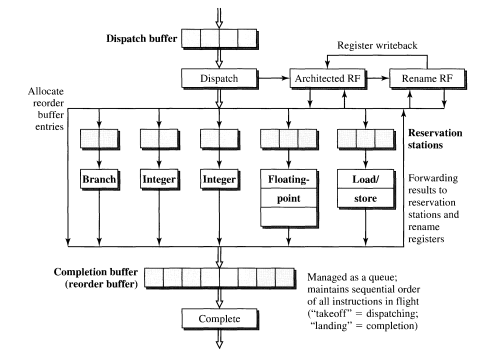
\includegraphics[scale=0.7]{DynExecCore.png}
    \caption{Dynamic Execution Core in a Superscalar OoO Processor \cite{shen_modern_2013}}
    \label{fig:hierarchy}
\end{figure}

Executing instructions in an order different from the original program order can lead to unexpected results due to dependencies among instructions (data-, name- and anti-dependencies). To enforce instruction dispatch (into the Functional Units) and instruction completion (to the \texttt{architectural register file}) in program order, additional buffers- \texttt{dispatch buffer} and \texttt{reorder buffer} respectively- are added to the pipeline. Further, to avoid errors due to name- and anti-dependencies (false dependencies), a separate \texttt{rename register file (RRF)} is used by the instructions to read from and write to when they are in-flight. When an instruction is completed by the \texttt{reorder buffer}, the data in the \texttt{RRF} is written back to the \texttt{architectural register file (ARF)}. Each Functional Unit includes a \texttt{reservation station (RS)}; instructions are issued to the Functional Units depending on the availability of the operands. 

\section{Dynamic Execution Core Simulator}
We implement a python-based Dynamic Execution Core Simulator with specialised Functional Units for Add/Store, Multiply, Divide and Load/Store instructions. An efficient implementation of branch instructions in the design would require a robust Branch Prediction Unit. As our focus here is dynamic execution of instructions, we leave out branch instructions from our design. The instruction set used by the simulator is specified in the problem statement (\href{https://github.com/aklsh/DynamicExecCore/blob/main/handout.pdf}{link}).

The functional units for Add/Store, Multiply and Divide are pipelined enabling a maximum throughput of one instruction per cycle regardless of the Functional Unit's latency. Further the reservation stations for these units issue instructions in an Out-of-Order manner depending on the availability of the operands.
The Load/Store unit processes instructions in a non-pipelined in-order manner.

The implementation details of rename registers, reservation stations, reorder buffers, functional units and the forwarding unit are described in the following section.
\section{Code Structure}
        \begin{compactitem}
        \item \texttt{class \textbf{regfiles}}
        \begin{compactitem}
            \item \texttt{class \textit{arfEntry}}: | data | busy | tag |
            \item \texttt{class \textit{arf}}: Architecture register file
            \item \texttt{class \textit{rrfEntry}}: | data | busy | valid |
            \item \texttt{class \textit{rrf}}: Rename register file
            \item \texttt{\textbf{destinationAllocate()}}: perform renaming for a given ARF register index.
            \item \texttt{\textbf{sourceRead()}}: return correct data (if available in ARF or RRF) or the appropriate RRF tag, and the validity of the data.
            \item \texttt{\textbf{registerUpdate()}}: update the data in the RRF upon finishing of instruction during forwarding and also update the ARF upon committing of instruction.
        \end{compactitem}
        \item \texttt{class \textbf{roBuffer}}
        \begin{compactitem}
            \item \texttt{class \textit{roBufferEntry}}: | busy | issued | finished | renameReg |
            \item \texttt{\textbf{updateState()}}: update the head and tail pointers of the ROB.
            \item \texttt{\textbf{insertEntry()}}: insert a new instruction in the ROB
            \item \texttt{\textbf{updateEntry()}}: update an instruction's entry on execution finish.
            \item \texttt{\textbf{complete()}}: commit the head instruction (if possible) and move the head pointer.
        \end{compactitem}
\begin{figure}[H]
    \centering
    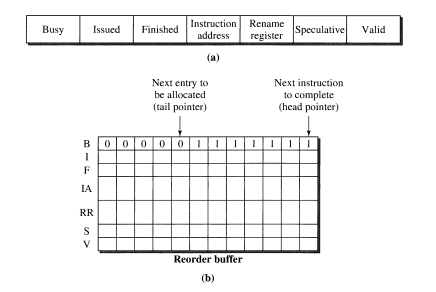
\includegraphics[scale=0.7]{RoB.png}
    \caption{Reorder Buffer Organisation \cite{shen_modern_2013}}
    \label{fig:hierarchy}
\end{figure}
        \item \texttt{\textbf{decode()}}: decode a given binary string into appropriate data fields - \texttt{r1}, \texttt{r2} etc.
        \item \texttt{\textbf{dispatch()}}: dispatch instructions from the dispatch buffer to the appropriate reservation stations. To enforce in-order dispatch, stall if necessary.
        \item \texttt{class \textbf{reservationStation}}
        \begin{compactitem}
            \item \texttt{class \textit{reservationStationEntry}}: | ID | Op1 | valid | Op2 | valid | ready | opcode |
            \item \texttt{\textbf{isFull()}}: return whether the RS is full or not
            \item \texttt{\textbf{addEntry()}}: add a new instruction to the reservation station
            \item \texttt{\textbf{updateEntries()}}: update the data and valid fields of the RS entries during forwarding
            \item \texttt{\textbf{putIntoFU()}}: push an instruction on the functional unit if it is ready.
        \end{compactitem}
\begin{figure}[H]
    \centering
    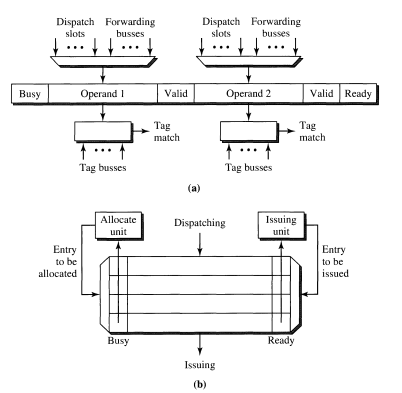
\includegraphics[scale=0.7]{RS.png}
    \caption{Reservation Station Organisation \cite{shen_modern_2013}}
    \label{fig:hierarchy}
\end{figure}        
        \item \texttt{class \textbf{\{AS/M/D\}U}}
        \begin{compactitem}
            \item \texttt{\textbf{shiftAndEval()}}: advance the various instructions in the unit to their next stages and return the finished computation data and tag for forwarding.
        \end{compactitem}
    \end{compactitem}
    To ensure that the load/store instructions are processed in-order, we implement slightly different functions and classes to take care of their extra fields in the instruction (3 operands, as opposed to 2) and to enforce in-order execution of the reservation station entries.
    \begin{compactitem}
        \item \texttt{class \textbf{LSreservationStation}}
        \begin{compactitem}
            \item \texttt{class \textit{LSrsEntry}}: | ID | Op1 | valid | Op2 | valid | offset | ready | opcode |
            \item \texttt{\textbf{isFull()}}: return whether the RS is full or not
            \item \texttt{\textbf{addEntry()}}: add a new instruction to the reservation station
            \item \texttt{\textbf{updateEntries()}}: update the data and valid fields of the RS entries during forwarding
            \item \texttt{\textbf{putIntoFU()}}: push an instruction on the functional unit if it is ready.
        \end{compactitem}
        \item \texttt{class \textbf{\{AS/M/D\}U}}
        \begin{compactitem}
            \item \texttt{\textbf{shiftAndEval()}}: advance the various instructions in the unit to their next stages and return the finished computation data and tag for forwarding.
        \end{compactitem}
    \end{compactitem}
    
    The config file (\texttt{conf.py}) is at the root of the directory. All necessary configuration parameters are highlighted here.
    
\section{Results}
Given are the cycle-by-cycle details provided by the simulator for some sample input test cases.

\begin{results}
    The functional units implemented in this simulator are pipelined and thus can have multiple instructions simultaneously executed, but in different stages of the pipeline. Thus, the reported cycles do not match with what is given as part of the sample test case provided as part of the problem statement.
\end{results}

\begin{table}[H]
\centering
\begin{tabular}{|c|c|}
\hline
\textbf{Test case} & \textbf{Cycles taken} \\ \hline
\texttt{ins.txt}            & 7            \\ \hline
\texttt{ins1.txt}           & 17           \\ \hline
\texttt{ins2.txt}           & 17           \\ \hline
\texttt{sample.txt}         & 27           \\ \hline
\end{tabular}
\caption{Cycles taken for different input test cases\tablefootnote{Test cases and corresponding output log files are present in the GitHub repository here - \href{https://github.com/aklsh/DynamicExecCore}{link}} }
\label{tab:results}
\end{table}

\begin{colorboxed}{\underline{Test Case 1:}}{sample.txt}{breakable}
    \inputminted[baselinestretch=0.85,breaklines]{text}{in/ins.txt}
    \hrule    
    \inputminted[baselinestretch=0.85,breaklines]{text}{out/insOut.txt}
\end{colorboxed}

%Beginning References. Don't add any text beyond this.
%------------------------------------------

%\newpage %sending References to the last page

\bibliography{references}
\bibliographystyle{acm}
\end{document}